\documentclass{standalone}
\usepackage{tikz}
\usepackage{graphicx}
\usepackage{pgf}
\usetikzlibrary{patterns}

\begin{document}

	

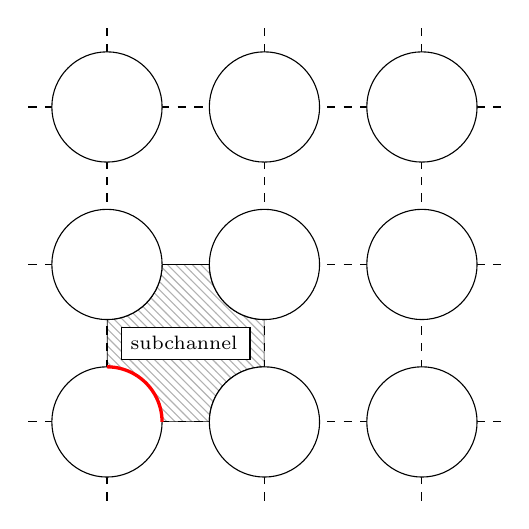
\begin{tikzpicture}
% define variables
\pgfmathparse{0.7}\let\r=\pgfmathresult
% fill subchannel with light blue
\begin{scope}
\clip (0,0) rectangle (2,2);
\draw[pattern=north west lines,pattern color=black!30] (0,0) rectangle (2,2) (0,0) circle[radius=\r] (0,2) circle[radius=\r]  (2,2) circle[radius=\r]  (2,0) circle[radius=\r];
\end{scope}

% draw grid
\foreach \y in {0, 2, 4}{
	\draw[dashed] (-1, \y)  -- (4+1.0, \y);
}
\foreach \x in {0, 2, 4}{
	\draw[dashed] (\x, -1)  -- (\x, 4+1.0);
}
% draw pins
\foreach \x in {0, 2, 4}{
\foreach \y in {0, 2, 4}{
	\draw[fill=white] (\x, \y) circle (\r);
}}

% highlight a pin subhcannel face (CTF face)
\draw [red,very thick,domain=0:90] plot ( {\r*cos(\x)}, {\r*sin(\x)} ) ;

% text
\node[draw, fill=white, text width=1.4cm] at (1,1) {\scriptsize subchannel};
\end{tikzpicture}



\end{document}
